\documentclass{beamer}

\usepackage[english]{babel}
\usepackage[utf8x]{inputenc}
\usepackage{tikz}
\usepackage{graphicx}
\usetikzlibrary{angles,quotes}

\title[Your Short Title]{word2vec - Word embeddings}
\author{Babak Maser, Hugo Platzer}
\date{October 23, 2018}

\begin{document}

\begin{frame}
  \titlepage
\end{frame}

\begin{frame}{Introduction: Natural language processing}

The processing of natural language is important for many applications, including the following:

\begin{itemize}
    \item Translation
    \item Sentiment analysis
    \item Web search
    \item Language modeling
\end{itemize}

Natural language processing (NLP) can analyze language
\begin{itemize}
    \item {\bf syntactically}: Parse grammar, check spelling etc.
    \item {\bf semantically}: Understand meaning, find synonyms etc.
\end{itemize}
\end{frame}



\begin{frame}{Vector space model}
In this model of information retrieval for NLP, documents are represented by a vector of the counts of terms occurring in them. Terms can be words, keywords or phrases. Vector operations can now be used to compare documents for similarity:

\centering
\vspace{1cm}
\begin{tikzpicture}
\coordinate (origin) at (0, 0);
\coordinate (P) at (2, 4);
\coordinate (Q) at (4, 2);
\draw[->] (origin) -- (P)  node[midway, label={[above, label distance=3mm] $v_1$}]{};
\draw[->] (origin) -- (Q)  node[midway, label={[below, label distance=-3mm] $v_2$}]{};
\draw pic["$\theta$", draw, <->, angle eccentricity=0.7, angle radius=1.5cm] {angle = Q--origin--P};

\draw node at (7, 2) {$\cos \theta = \frac{v_1 \cdot v_2}{||v_1|| \  ||v_2||}$};
\end{tikzpicture}
\end{frame}


\begin{frame}{Vector Representation of word}
\textbf{one-hot representation:} \\
 The dimension of each word would be the number of unique words in the corpus.\\
$\qquad$
  $\qquad$  Book = [ 0 0 0 1 0 0 0 0 0 0 0 0 0 0 0  ]
\\
\textbf{Co-occurance Matrix:} \\
 $\qquad$ Silence is the language of God, all else is poor translation. (Rumi 1207 , 1273)
 
\begin{center}
\begin{tabular}{ |c|c|c|c|c| } 
 \hline
          & Silence & is & language & God \\ 
 Silence  & 0 & 1 & 0  & 0 \\ 
 is       & 1 & 0 & 0 & 0  \\ 
 language & 0 & 1 & 0 & 0  \\ 
 God      & 0 & 0 & 1 & 0 \\ 
 \hline
\end{tabular}
\end{center}
 


\end{frame}


\begin{frame}{Word2vec}
Word2vec is a language model that learns about the relationship between words. The output vectors show interesting relationships, e. g:

$$vec("king") - vec("man") + vec("woman") \approx vec("queen").$$

The model should put words that occur in similar context into clusters:
\end{frame}

\begin{frame}{Word2vec}

\centering

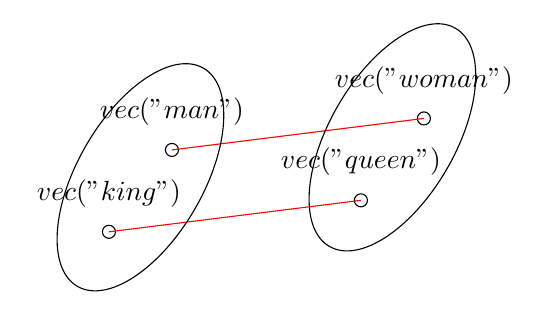
\begin{tikzpicture}[scale=0.8]
\node[draw, circle, scale=0.5, label = {[label distance=1mm] $vec("king")$}] at (0, 0) {};
\node[draw, circle, scale=0.5, label = {[label distance=1mm] $vec("man")$}] at (1, 1.3) {};
\node[draw, circle, scale=0.5, label = {[label distance=1mm] $vec("queen")$}] at (4, 0.5) {};
\node[draw, circle, scale=0.5, label = {[label distance=1mm] $vec("woman")$}] at (5, 1.8) {};
\draw[red] (0, 0) -- (4, 0.5);
\draw[red] (1, 1.3) -- (5, 1.8);
\draw[rotate around={-30:(0, 0)}] (0, 1) ellipse (1cm and 2cm);
\draw[rotate around={-30:(4.5, 1.5)}] (4.5, 1.5) ellipse (1cm and 2cm);
\end{tikzpicture}

\vspace{1em}
$dist(vec("king"), vec("man")) \approx dist(vec("queen"), vec("woman"))$

$\Rightarrow vec("king") - vec("man") \approx vec("queen") - vec("woman")$

$\Rightarrow vec("king") - vec("man") + vec("woman") \approx vec("queen")$.
\end{frame}

\begin{frame}{Word2vec}

Methods :
\begin{itemize}
\item 
CBOW (Continuous Bag of words)
\item
Skip-Gram
\end{itemize}

The CBOW architecture predicts the current word based on the context. \\
The skip-Gram predicts surrounding words given the current words.


\end{frame}




\begin{frame}{The skip-gram model}
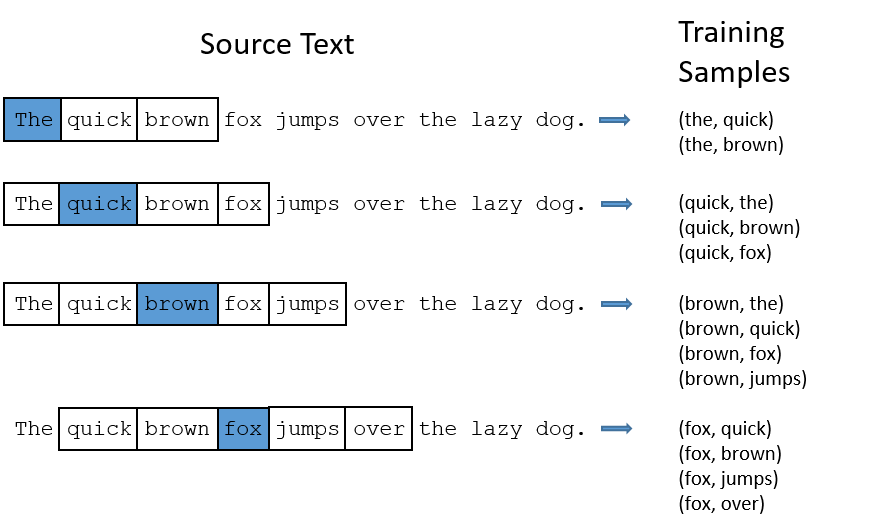
\includegraphics[width=\textwidth]{training_data.png}
\end{frame}


\begin{frame}{The skip-gram model}
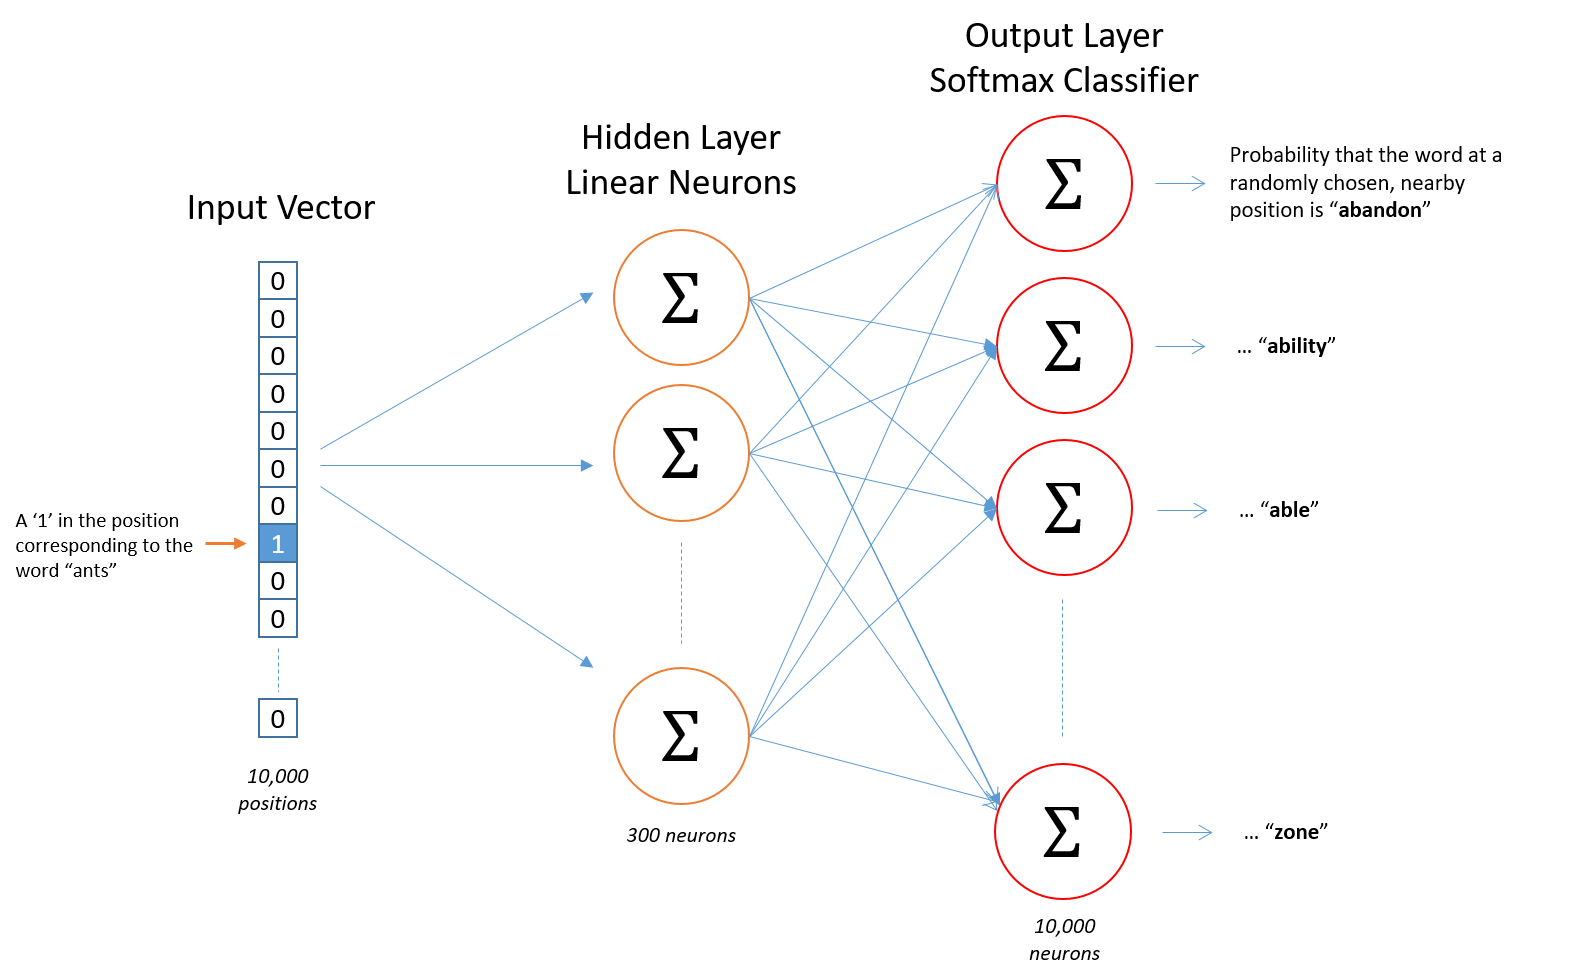
\includegraphics[width=\textwidth]{skip_gram_net_arch.png}
\end{frame}


\begin{frame}{The continuous-bag-of-words model}
\begin{itemize}
    \item The skip-gram model tries to guess context words based on the current word, the CBOW model goes the other way
    \item The one-hot vectors of the surrounding words are summed up (counting the context words), the order of the words is not considered, this is the network input
    \item The current word's one-hot vector is the desired output
\end{itemize}

\end{frame}













\begin{frame}{Next steps}
\begin{itemize}
\item Choose a minimal, but interesting corpus of English words

\item Select a source of text to train the network from
    \begin{itemize}
        \item Browse through Wikipedia or similar websites
        \item Extract long enough passages only consisting of our limited vocabulary
    \end{itemize}

\item Generate skip-gram or CBOW pairs for network training

\item Desired size of word vector / hidden layer size

\item Potential problems with network training (large number of weights)

\item Use test data to check prediction accuracy, adjust training parameters if necessary
\end{itemize}
\end{frame}


\end{document}
